\chapter{Planilla Base}

La \textit{Planilla Base} tiene como objetivo controlar la información y la gestión de los análisis de parámetros y estaciones. En ella se determinan los nombres de estaciones, códigos de contenedores, matrices físicas asignadas a cada parámetro y los laboratorios que realizan cada análisis, entre otros datos.

La responsabilidad del llenado correcto de la información recae en los siguientes usuarios:

\begin{itemize}
	\item \textbf{Jéfe de Proyecto}: asigna el laboratorio que analizará parámetro e ingresa información económica.
	\item \textbf{Jéfe de Área}: comprende la tarea de mayor complejidad en cuanto a la cantidad de información, determina a partir de la propuesta de proyecto las estaciones y parámetros.
	\item \textbf{Asistente Químico}: Completa en cuadro 1 la zona asignada.
	\item \textbf{Asistente de Logística}: Completa en cuadro 1 la zona asignada
\end{itemize}

La hoja llamada \textit{Labs} debe ser completada añadiendo o actualizando la información de cada laboratorio en particular, es necesario que este siempre \textbf{actualizada} y con los datos correctos, ya que el sistema de automatización toma esta lista como principal referente para asignar los documentos resultantes. Ver figura \ref{pb_labs}.

\begin{landscape}
\begin{figure}
	\centering
	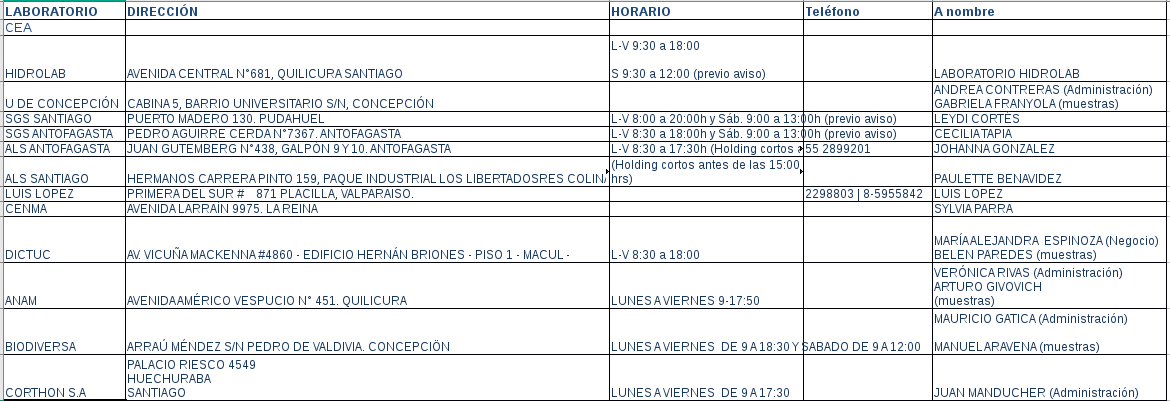
\includegraphics[scale=.6]{pb_labs.png}
	\caption{Tabla Información de Laboratorios}
	\label{pb_labs}
\end{figure}
\end{landscape}
	
La hoja de \textit{Parametros} contiene la lista de todos los parámetros de los cuales se pueden hacer análisis, la información debe estar actualizada y deben revisarla el Jéfe de Proyecto o el Jéfe de Área antes de completar la planilla base en hoja \MakeUppercase{base\_sse}, de la manera que se observa en figura \ref{pb_param}.

\begin{figure}
	\centering
	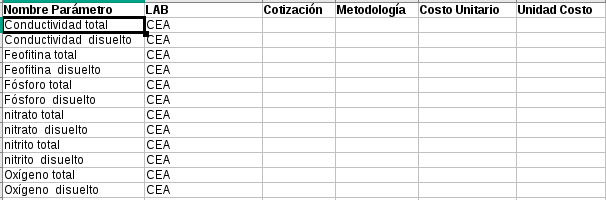
\includegraphics[scale=.6]{pb_param.png}
	\caption{Tabla Información de Parámetros}
	\label{pb_param}
\end{figure}

La hoja de \textit{Matrices} contiene la relación entre matrices de agua con de sedimentos, mostrando las únicas posibilidades de combinación en la misma estación, solo pueden existir combinaciones en que la relación sea '1', como se ve en la figura \ref{pb_matrices} .

\begin{figure}
	\centering
	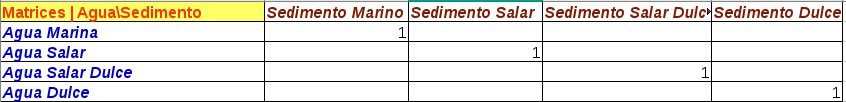
\includegraphics[scale=.6]{pb_matrices.png}
	\caption{Tabla relación de matrices físicas agua-sedimento}
	\label{pb_matrices}
\end{figure}

A continuación se hará un análisis exploratorio por cada sección de la planilla, explicando la información requerida y condiciones de validación.

\section{Explorando la Planilla Base}

Puedes descargar la planilla base desde \href{http://www.mediafire.com/view/levr2xh9bytaki2/Patron_FL.xlsx}{Planilla Base}

\subsection{Encabezado}

\textbf{Usuario Responsable:} Jéfe de Área

Debe asignar una numeración única a la planilla de solicitud de servicio.

\subsection{Antecedentes}

\textbf{Usuario Responsable:} Jéfe de Proyecto

Se debe completar la información del proyecto (nombre y código), del Jefe de Proyecto, Área que solicita, fecha de solicitud y entrega. La diferencia entre ambas fechas debe ser de al menos 45 días continuos. La tabla se puede ver en \ref{pb_antecedentes}.

\begin{figure}
	\centering
	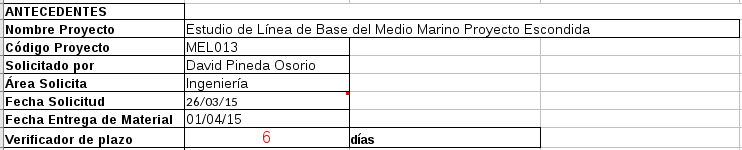
\includegraphics[scale=.7]{pb_antecedentes.png}
	\caption{Tabla de antecedentes en planilla base}
	\label{pb_antecedentes}
\end{figure}
 
\subsection{Parámetros} 

\textbf{Usuarios Responsables:} \{Jéfe de Proyecto, Jéfe de Área, Asistente Químico y Asistente de Logística\}

Cada usuario debe completar el área correspondiente asignada y enunciada en cada sector.

\subsubsection{Responsabilidad de Jéfe de Proyecto}

Este usuario debe extraer la información de la propuesta técnica del proyecto y listar lo
siguiente:

\begin{itemize}
 \item Parámetros
 \item Cantidad de estaciones por parámetro
 \item Réplicas por parámetro
 \item Matriz relacionada a parámetro
 \item Metodología de análisis de parámetro 
 \item Límite de detección especificada en propuesta técnica
\end{itemize}

En este sector la información particular es 'Parámetro' de aquí se debe definir el resto de los valores relacionados a este parámetro, esto se puede observar en la tabla de 'Jéfe de Proyecto' en figura \ref{pb_parametro_jp}

\begin{landscape}	 
\begin{figure}
	\centering
	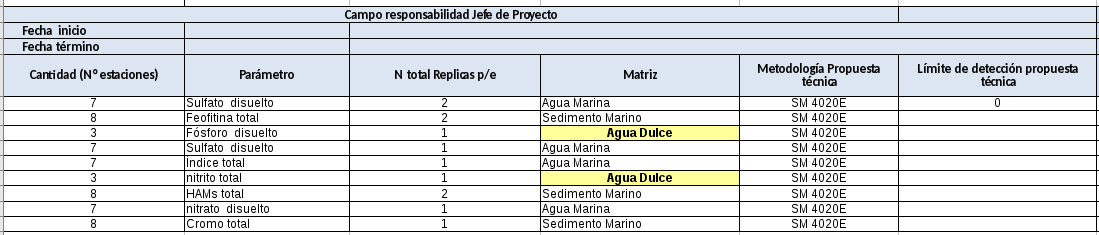
\includegraphics[scale=.6]{pb_parametro_jp.png}
	\caption{Tabla de parámetros Jéfe de Proyecto}
	\label{pb_parametro_jp}
\end{figure}
\end{landscape}

\subsubsection{Responsabilidad de Jéfe de Área}

Este usuario debe evaluar técnica y económicamente el análisis a realizar de cada parámetro y asignar correspondientemente cada laboratorio, además de ingresar los costos, entre ello lo siguiente:

\begin{itemize}
	\item Fecha Inicio
	\item Fecha Término
	\item Laboratorio
	\item Grupo
	\item Código de Contenedores
	\item Cotización
	\item Costo
	\item Unidad de costo (moneda)
\end{itemize}

La tabla se puede observar en la figura \ref{pb_parametro_ja}

\begin{figure}
	\centering
	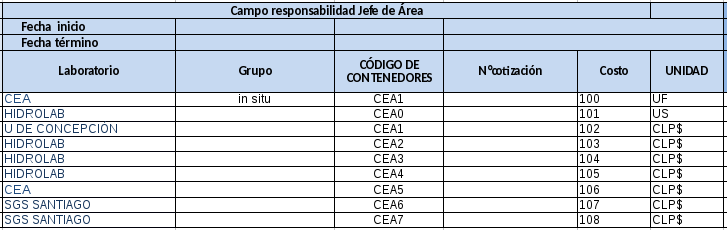
\includegraphics[scale=.8]{pb_parametro_ja.png}
	\caption{Tabla de parámetros Jéfe de Área}
	\label{pb_parametro_ja}
\end{figure}

La información del nombre de Laboratorio debe de tener el \MakeUppercase{mismo nombre} de la hoja \textit{Labs}.

\subsubsection{Responsabilidad de Asistente Químico}

El asistente químico completa la información respecto al envío de las ordenes de compra, tal como se observa en la tabla de la figura \ref{pb_parametro_aq}

\begin{figure}
	\centering
	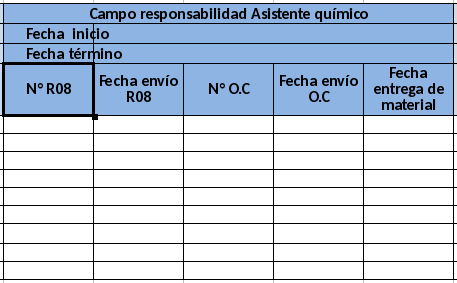
\includegraphics[scale=.6]{pb_parametro_aq.png}
	\caption{Tabla de parámetros Asistente Químico}
	\label{pb_parametro_jq}
\end{figure}

\subsubsection{Responsabilidad de Asistente de Logística}

El asistente químico completa la información respecto a la recepción de materiales y equipos, tal como se observa en la tabla de la figura \ref{pb_parametro_al}

\begin{figure}
	\centering
	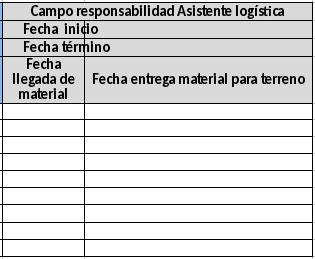
\includegraphics[scale=.6]{pb_parametro_al.png}
	\caption{Tabla de parámetros Asistente de Logística}
	\label{pb_parametro_al}
\end{figure}

\subsection{Relación Código Estación con Matriz Física} 

Consiste en una tabla que tiene en el encabezado de las columnas los nombres de matrices físicas y en la primera columna los nombres de cada estación. Cada celda relacionada debe llenarse con \textbf{1} sí y solo sí existe extracción de parámetros en esa estación - matriz. No completar con ningún otro valor el resto de las celdas.

Se puede observar la tabla en la figura \ref{estacion_matriz}

\begin{landscape}
\begin{figure}
	\centering
	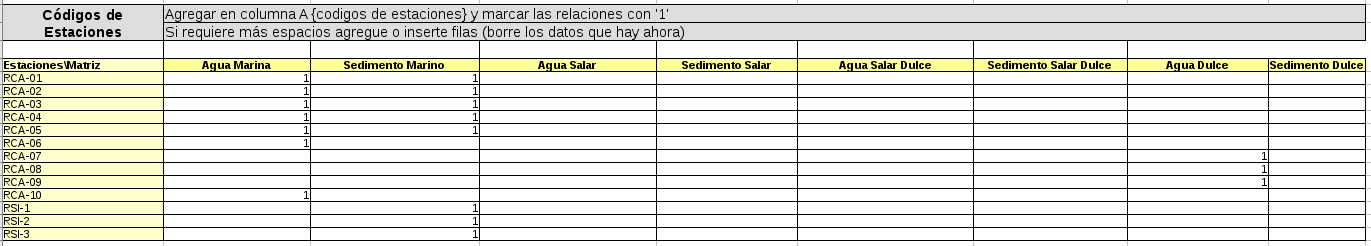
\includegraphics[scale=.6]{estacion_matriz.png}
	\caption{Tabla de relación Estación-Matriz Física}
	\label{estacion_matriz}
\end{figure}
\end{landscape}

\subsection{Materiales y Equipos}

\textbf{Usuario Responsable:} Jéfe de Proyecto

Esta tabla se completa con la cantidad de elementos (equipos o materiales) y los nombres (como se observa en figura de tabla \ref{material_equipo}), se determina en base al método de extracción de cada parámetro, ya que cada uno requiere uno u otro equipo determinado.

\begin{figure}
	\centering
	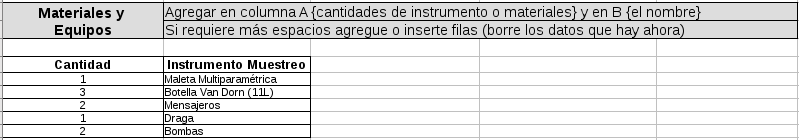
\includegraphics[scale=.6]{material_equipo.png}
	\caption{Listado de materiales y equipos}
	\label{material_equipo}
\end{figure}


\subsection{Observaciones}

\textbf{Usuario Responsable:} Jéfe de Proyecto

Las observaciones van relacionadas a cada documento (según laboratorio) y matriz (necesariamente para el FL33, como se ve en figura \ref{observaciones}). Cada celda puede ser llenada con varias líneas (en la misma celda).

\begin{landscape}
\begin{figure}
	\centering
	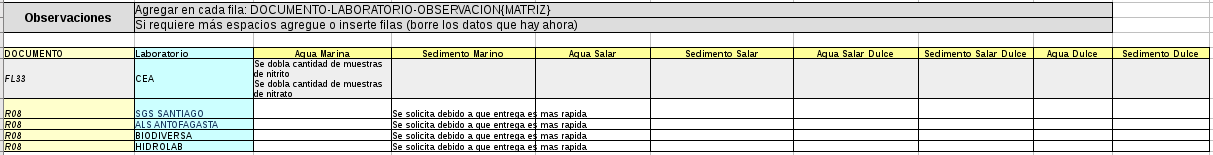
\includegraphics[scale=.6]{observaciones.png}
	\caption{Tabla de observaciones}
	\label{observaciones}
\end{figure}
\end{landscape}

\subsection{Adjuntos a R08} 

\textbf{Usuario Responsable:} Jéfe de Proyecto

Completar solo con \textbf{si} en caso de que se añadan documentos adjuntos a la solicitud relacionada con laboratorio.

\begin{figure}
	\centering
	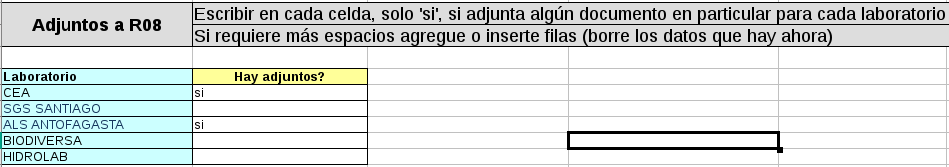
\includegraphics[scale=.6]{adjuntos.png}
	\caption{Tabla de documentos adjuntos}
	\label{adjuntos}
\end{figure}